\documentclass[paper=a4,fontsize=11pt,DIV=8,BCOR=5mm,twoside,pdftex]{scrartcl}

\usepackage[pdftitle={Greedily maximizing social influence},
pdfauthor={Christian Ali Mehmeti-Göpel},
pdfborder={0 0 0}]{hyperref}
\title{Greedily maximizing social influence}
\usepackage[english]{babel}
\usepackage{amsmath,amssymb,amstext,amsthm}
\usepackage[utf8]{inputenc}
\usepackage{cite}
\usepackage{algorithmicx}
\usepackage{algorithm}
\usepackage{afterpage}
\usepackage{lmodern}
\usepackage{microtype}
\usepackage{algpseudocode}  
\usepackage{tikz}
\usepackage{pgfplots}

\newcommand\blankpage{%
	\null
	\thispagestyle{empty}%
	%	\addtocounter{page}{-1}%
	\newpage}

\swapnumbers

\setlength{\parindent}{0ex}


\begin{document}
	\maketitle
In this document we present the results of some experimentation with the algorithm presented in the paper "Maximizing the Spread of Influence through a Social Network" by Kempe / Kleinberg / Tardos.
	
	\section{Implementation}

Let $G = (V, E)$ be the graph we want to analyze. Let $A\subseteq V$ be the output of the algorithm, the subset of nodes we will target. Let $k := |A|$ be the size of the desired initial active node set. Let $\sigma(A)$ be the expected number of nodes that are activated after a simulation with the cascade / linear threshold model, given the initial set $A$.\\

The algorithm starts with an empty set, and adds at each iteration a node to the set $A$ : it choses greedily the node that, if added to $A$, increments the most our objective function $\sigma(A)$ in this step. Because we cannot evaluate the expected value analytically, we simulate the process $num\_sim$ times, and approximate the expected value with the average value.  \\

The pseudocode of the algorithm is the following : 

\begin{algorithm}[H]
	\caption{Greedy Algorithm}
	\begin{algorithmic}
		\State{$A := \emptyset$}
		\While{$|A| < k$}
			\For{all nodes $v \in V \setminus A$}
				\For{$num\_sim$ iterations}
					\State{Simulate IC / LT with initial nodes $A\cup v$}

				\EndFor
				\State{Calculate an average activation score for $v$}	
			\EndFor
			\State{Determine the node $v$ with the highest average score}
			\State{Set $A$ := $A\cup v$}
		\EndWhile \\
		\Return{$A$}
	\end{algorithmic}
\end{algorithm}

Obviously, the algorithm can produce different results whether used with the linear threshold model or with the independent cascade model.

\section{Graph Used}

We used an undirected graph of anonymized facebook data, with $|V| = 52$ and $|E| =292 $.

\section{Results}	
	
We first observe how $\sigma(A)$ increases in both models when we allow for a bigger size $k$ of the initial set. We use $num\_sim = 100000 $ as in the paper.\\

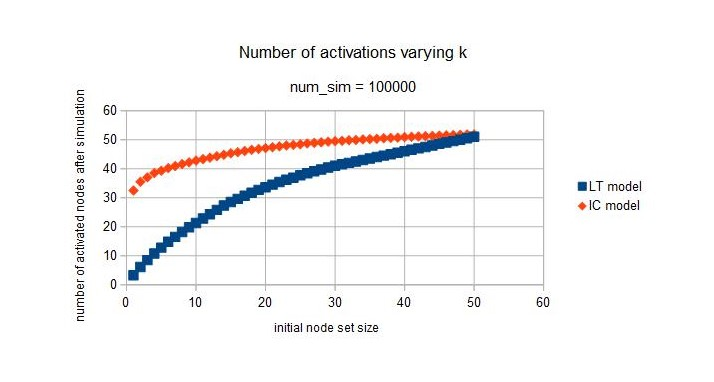
\includegraphics[height=8cm]{var_k.jpg}

We then want to analyze how imprecise the approximated value of $\sigma(A)$ is when $num\_sim$ is low. We find that on our graph, even with only 10 simulations, the estimation is quite near the value for 100000 simulations.\\

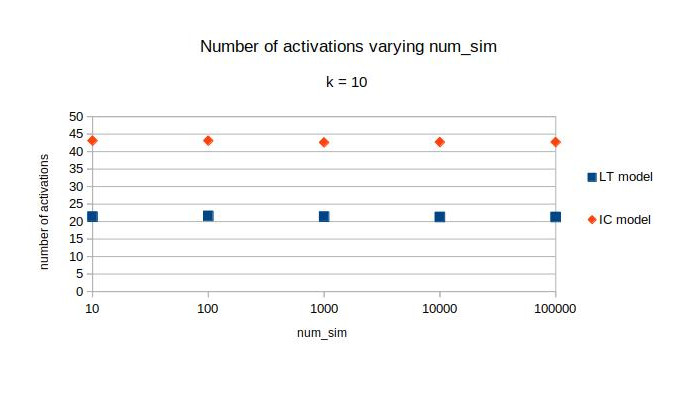
\includegraphics[height=8cm]{var_numsim.jpg}

\end{document}